\documentclass[11pt,aspectratio=169]{beamer}
\usepackage{amsmath,amssymb,booktabs,array,graphicx}
\usepackage{attachfile2}
\renewcommand{\familydefault}{\sfdefault}
\definecolor{Navy}{HTML}{142E45}
\definecolor{Teal}{HTML}{087E8B}
\definecolor{Ink}{HTML}{243746}
\definecolor{Muted}{HTML}{586A75}
\setbeamercolor{normal text}{fg=Ink,bg=white}
\setbeamercolor{frametitle}{fg=Navy,bg=white}
\setbeamercolor{structure}{fg=Teal}
\setbeamercolor{title}{fg=Navy}
\setbeamerfont{frametitle}{size=\Large,series=\bfseries}
\setbeamerfont{normal text}{size=\normalsize}
\setbeamertemplate{navigation symbols}{}
\setbeamertemplate{itemize items}[circle]
\setbeamertemplate{frametitle}{\vspace{0.24cm}\insertframetitle\par\vspace{0.08cm}}
\setbeamertemplate{footline}{\hspace{0.55cm}\color{Muted}\fontsize{7}{8.5}\selectfont CS 74\hfill Emilio Sebastian Daza Vigo\hfill\insertframenumber/5\hspace{0.55cm}\vspace{0.16cm}}
\setbeamersize{text margin left=0.6cm,text margin right=0.6cm}
\setlength{\tabcolsep}{5pt}
\newcommand{\source}[1]{\par\vfill{\color{Muted}\fontsize{7}{8.5}\selectfont #1\par}}
\newcommand{\topic}[1]{\par{\color{Teal}\bfseries #1}\par\vspace{0.12cm}}
\newcommand{\tightlist}{\setlength{\itemsep}{0.17cm}\setlength{\parskip}{0pt}}
\hypersetup{pdftitle={Learning Corrections to Drone Motion Models},pdfauthor={Emilio Sebastian Daza Vigo},colorlinks=true,urlcolor=Teal}
\begin{document}

\begin{frame}[t]{Learning corrections to drone motion models}
\par\vspace{0.32cm}
\topic{Research question}
When does a neural correction to a simple thrust model improve acceleration predictions on unseen flights?
\par\vspace{0.22cm}
\[
\underbrace{\widehat{\mathbf a}_{\mathrm{res}}(\mathbf x)}_{\text{body-frame prediction}}
=
\underbrace{(0,0,c\!\sum_{j=1}^{4}\Omega_j^2)}_{\text{fitted thrust model}}
+
\underbrace{f_\theta(\mathbf x)}_{\text{learned correction}}
\]
\par\vspace{0.20cm}
The models use body velocity, angular velocity, and four squared rotor speeds to predict three components of body-frame acceleration.
\par\vspace{0.22cm}
I compare the models on recorded flights and test how the learned estimates affect tracking in simulation.
\source{Flight data and model inspiration from Bauersfeld et al., NeuroBEM, RSS 2021. \href{https://doi.org/10.15607/RSS.2021.XVII.042}{doi:10.15607/RSS.2021.XVII.042}.}
\end{frame}

\begin{frame}[t]{Flight splits and model training}
\par\vspace{-0.08cm}
\begin{center}
\begin{tabular}{lrrr}
\toprule
 & Training & Validation & Test \\
\midrule
Original flights & 65 & 17 & 13 \\
Retained observations & 157,092 & 35,590 & 32,234 \\
\bottomrule
\end{tabular}\par
\end{center}
\par\vspace{0.06cm}
\begin{columns}[T,onlytextwidth]
\begin{column}{0.48\textwidth}
\topic{Data preparation}
\begin{itemize}\tightlist
\item Keep all segments of each flight together. Hold out every flight in the authors' test list.
\item Retain every eighth row and fit the scaler on the training set.
\item Use validation RMSE to select the ridge penalty and network checkpoints.
\end{itemize}
\end{column}
\begin{column}{0.48\textwidth}
\topic{Models and training}
Thrust, ordinary least squares, ridge, direct MLP, residual MLP.
\par\vspace{0.18cm}
Both MLPs use 32 ReLU units. Adam uses a $10^{-3}$ learning rate and batches of 256, for up to 50 epochs with patience 5.
\par\vspace{0.18cm}
Paired seeds 42, 43, and 44. Ridge $\alpha\in\{1,100,10{,}000\}$.
\end{column}
\end{columns}
\source{I used a notebook viewer in place of Streamlit and added a control study in Isaac Sim. The flight split uses seed 42.}
\end{frame}

\begin{frame}[t]{Residual prediction helps at higher speeds}
\begin{columns}[T,onlytextwidth]
\begin{column}{0.48\textwidth}
\topic{All held-out observations}
\begin{tabular}{lr}
\toprule
Model & RMSE \\
\midrule
Thrust & 1.7365 \\
OLS & 0.8783 \\
Ridge & 0.9193 \\
Direct MLP & $0.4985\pm0.0092$ \\
Residual MLP & $\mathbf{0.4906}\pm0.0178$ \\
\bottomrule
\end{tabular}\par
\par\vspace{0.16cm}
{\small RMSE is in $\mathrm{m/s^2}$. The $\pm$ values show sample standard deviation across three training seeds.}
\end{column}
\begin{column}{0.48\textwidth}
\topic{Test error by speed}
\begin{tabular}{lrr}
\toprule
Speed & Direct & Residual \\
\midrule
$<5$ m/s & $\mathbf{0.3322}$ & 0.3369 \\
$\geq5$ m/s & 0.6963 & $\mathbf{0.6772}$ \\
\bottomrule
\end{tabular}\par
\par\vspace{0.18cm}
At 5 m/s and above, the residual model lowers RMSE by \textbf{2.7\%} relative to direct prediction.
\par\vspace{0.16cm}
{\small Slow: 20,350 observations from 13 flights.\par
Fast: 11,884 observations from 12 flights.\par
A flight may contribute to both groups.}
\end{column}
\end{columns}
\par\vspace{0.16cm}
In an exploratory comparison, residual prediction lowered RMSE on \textbf{10 of 12 flights} with samples at 5 m/s or faster.
\source{NeuroBEM test results. RMSE is the square root of the mean squared error across observations and acceleration axes.}
\end{frame}

\begin{frame}[t]{Braking and gust recovery in Isaac Sim}
\begin{columns}[T,onlytextwidth]
\begin{column}{0.73\textwidth}
\vspace{0.05cm}
\centering
\href{run:media/drone_demo.mp4}{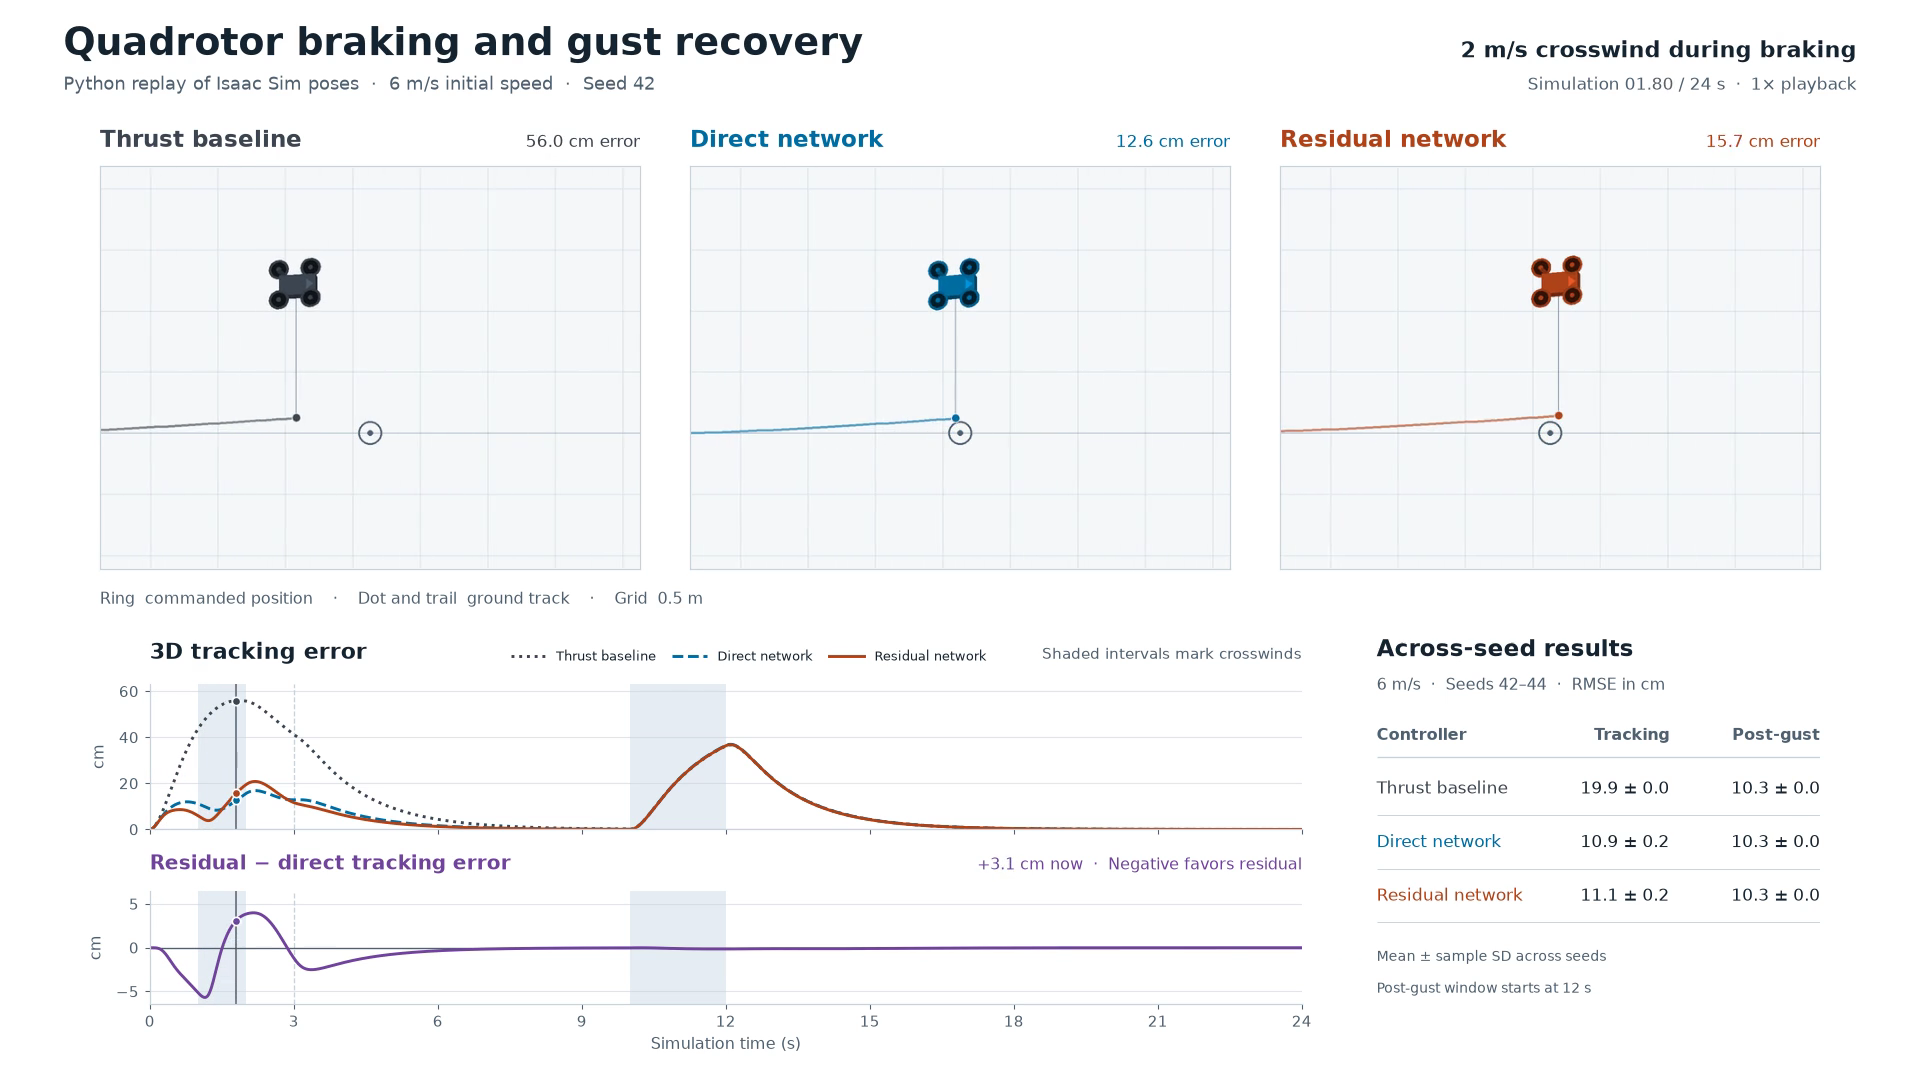
\includegraphics[width=0.90\linewidth]{figures/snapshot_braking_gust.png}}
\par\vspace{0.08cm}
\textattachfile[mimetype=video/mp4,description={Isaac Sim drone demo, 13.2 seconds},color=0.03 0.49 0.55]{\detokenize{media/drone_demo.mp4}}{\footnotesize\bfseries 13.2 s replay with quiet hover at $4\times$}
\end{column}
\begin{column}{0.245\textwidth}
{\small\color{Teal}\bfseries Tracking RMSE}\par
{\footnotesize 6 m/s, three seeds}\par\vspace{0.12cm}
{\small Thrust: 19.89 cm\par
Direct: \textbf{10.85 cm}\par
Residual: 11.10 cm}\par\vspace{0.22cm}
{\footnotesize\textbf{Errors converge during the hover gust.}\par\vspace{0.13cm}
All controllers share a drag model. Learned corrections act laterally.}
\end{column}
\end{columns}
\source{Isaac Sim 6.2 (PhysX) computed the motion. Python replays the saved 6 m/s trial (seed 42).}
\end{frame}

\begin{frame}[t]{Conclusions and future work}
\topic{What the comparisons show}
The residual model predicts acceleration slightly better at 5 m/s and above. The direct model does better at lower speeds and has lower mean tracking error in the simulation.
\par\vspace{0.22cm}
\topic{Next experiments}
\begin{itemize}\tightlist
\item Repeat model selection with cross-validation grouped by flight and test on new recording sessions.
\item Compare explicit drag terms with learned corrections at similar model capacity and examine the error for each flight.
\item Check coordinate conventions and prediction uncertainty before comparing the controllers on real flights.
\end{itemize}
\source{\textbf{AI disclosure}\enspace GPT assisted residual-learning concepts and Isaac Sim use through Dartmouth Clusters\par
Related control work: Torrente et al., Data-Driven MPC for Quadrotors, RA-L 2021, \href{https://doi.org/10.1109/LRA.2021.3061307}{doi:10.1109/LRA.2021.3061307}.}
\end{frame}
\end{document}
